\subsection{Instruction Solver}
An instruction is composed of three fields: {\tt opcode}, {\tt operand} and {\tt modifier}. An operand can be register, constant memory, global memory, shared memory, immediate, or predicate register.
The encoding of operand can be inferred by its name. For instance, the register operand {\tt R5} might be
inferred as $101$ in binary format, immediate $0x9$ is $1001$. Besides, the fixed lengths of these fields allow us to determine their positions and lengths and hence encoding. Encodings of opcode and modifier are mnemonic symbols, therefore, they can not be speculated by names. Modifiers are instruction specific, the same kind of modifier can be different encodings for different instructions. For instance, masks of type-size
modifier for {\tt LD} and {\tt LDG} are at different positions. So we deal with modifier for each instruction separately. 

\subsubsection{Operand:Fixed Length Field}
Algorithm~\ref{algo:int_solver} shows pseudocode for immediate typed operand decoding process. 
The basic idea is that match binary encoding of operand in $64$ instruction encoding and find
position until the postion is unique. The input instructions are from disassembly code (i.e., NVIDIA CUBLAS library).
First, we randomly pick up an instruction that has the field we want to probe, and represent the field in binary by its name. Second, we match the operand binary in $64$-bit instruction encoding, and find possible positions. Third, we intersect current candidates with previous ones, if the number of candidates is $1$, we find the position. Otherwise, we set the current candidate to the previous one and randomly pick next instruction to repeat the procedure.
Other operand type such as register operand can be use similar routine by matching the corresponding operand binary.

\begin{algorithm}
      \caption{Immediate Solver}
      \label{algo:int_solver}
  \begin{algorithmic}[1]
	  \State \textbf{input:} instMap
      \State \textbf{output:} pos, length
      \State $currPos$ $\gets$ \{\}
      \State $prePos$ $\gets$ \{0,1,2,...63\}
	  \LineComment {check if position is unique}
      \While {length($prePos$) != 1}
	  \LineComment {fetch a instruction with this field}
      \State $inst$ $\gets$ $instMap[random()]$
      \If {$inst.src1type$ == $imm$}
      \State $instEnc$ $\gets$ inst->enc64
	  \LineComment {express immediate in completement code}
      \State $immBin$ $\gets$ completement($imm$)
      \State $pos$ $\gets$ 0
      \State $immLen$ $\gets$ length($immBin$)
      \LineComment {match immBin in 64 bit encoding}
      \While {$pos$+ $immLen$ < $64$}
      \If {strcmp($immBin,instEnc+pos,immLen$)}
      \LineComment {find all the possible positions}
      \State pushback(currPos, pos)
      \EndIf
      \EndWhile
      \LineComment {common position between curPos and prePos}
      \State $currPos$ $\gets$ $curPos$ $\cap$ $prePos$
      \State $prePos$ $\gets$ $currPos$
      \State $currPos$ $\gets$ \{\}
      \EndIf
      \EndWhile
      \State return $prePos[0]$
  \end{algorithmic}
\end{algorithm}

Once operand position is found, we need to probe or verify the length of operand encoding. Some are easy to be
deduced, for example, each thread can use at most $256=2^{8}$ registers, we could predict the length of register operand mask to be $8$.
However, other operand types like immediate $0x48$ or subscript of constant memory $C[0x2][0x05]$, are more complicated to predicate. Our solution is to set the bit from the position bit by bit to check whether the operand value is grown as we expected. For instance, by using Algorithm~\ref{algo:int_solver}, we find out that the immediate operand position of {\tt IADD RX, RY, 0ximm} (the RX and RY are arbitrary register operands, 0ximm is immediate operand) is at bit $23$ as shown in Figure~\ref{fig:imm}. As specified in~\cite{cuda2015programming}, NVIDIA GPU uses little-endian representation, then we set the bits higher than the $23$ to $1$ bit by bit, and observe the the disassembled code. Immediate value increases continuely until reaches value {\tt 0x7ffff}, which means that $41\sim23$ is for integer immediate. No {\tt fffff} immediate was got even if we set bit $42$ to be $1$.  

\begin{figure}[htbp]
\begin{center}
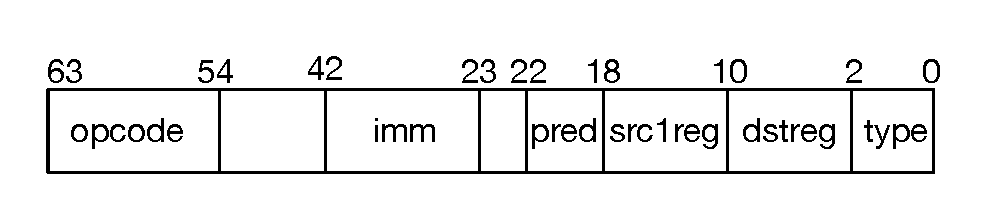
\includegraphics[scale=0.5]{imm}
    \caption{Immediate position at {\tt IADD} instruction}
\label{fig:imm}
\end{center}
\end{figure}

\subsubsection{Opcode}
Unlike operand, opcodes and modifiers do not show their encodings literally. One possible way to crack the operand encoding is to write intermediate codes
based on NVIDIA PTX syntax, and generate encoding by using NVDIA toolchain.
Then, opcode can be got by stripping out operand mask, and flag can be found by stripping out both opcode and operand mask. However, the uncompleteness of NVIDIA document hinders us to find out all the opcodes and instruction modifiers. Another feasible way is to emulate all of possible binary combinations after striping out operand mask.
In general, each instruction has $3$ register operands, and one $4-bit$ predicate register, $64-8*3-4=36$ bits are left to probe.
In fact, we can further prune the search space by recognizing possible position by algorithm~\ref{algo:opcode}. By randomly probing bit by bit, we find that both the top $10$ bits and lower $2$ bits represent opcode and other bits represent flags. Thus, we only enumerate these opcode bits which generate a acceptable search space. Finally, we find the minimal opcode without any flags. 


\begin{algorithm}
      \caption{Opcode Solver}\label{algo:opcode}
  \begin{algorithmic}[1]
      \State \textbf {input:} instMap
      \State \textbf {onput:} pos
      \For {$i \gets 0, N$}
	  \LineComment {fetch a instruction from generated database}
      \State $enc \gets instMap[i]$ 
	  \LineComment {check if bit j represent opcode}
      \For {$j \gets 0, 63$}
	  \LineComment {if bit j is not operand and value is 0}
      \If {notOprd($enc[j]$) and $enc[j] == 0$}
      \State newCode = setbit($enc[j], j, 1$)
	  \LineComment {disassemble newCode to get newInst}
      \State newInst=nvdisasm(newCode)
	  \LineComment {if opcode is changed, bit j represents opcode}
      \If {$newInst.op\neq oldInst.op$}
      \State pushback($pos$,$j$)
      \EndIf
      \EndIf
      \EndFor
      \EndFor
      \State return pos
  \end{algorithmic}
\end{algorithm}

\subsubsection{Modifier: Instruction Specific}

Modifier(also called flags) defines a specific behavior for an instruction. For example,
{\tt LD} instruction has type-size modifiers, such as {\tt .u8}, {\tt .s8}, {\tt .u16}, {\tt .32}, {\tt .64} and {\tt .128}. {\tt LD} also has cache operation modifier, such as {\tt .ca}(cache at all level) and {\tt .cg}(cache at global level). Modifiers are much more complicated because its position spans accross the reminding bits and one instruction may have more than one kinds of modifiers. By excluding both opcode and operand mask, there remain around $24$ bits. In order to reduce search space, we observe that the default value for modifier is $0$. That is, modifier works when at least one bit is set. We can check possible positions of modifiers by greedily set the remaining bits one by one to observe whether flags will change.
